\documentclass[12pt,a4paper]{article}
\usepackage[utf8]{inputenc} 
\usepackage[T1]{fontenc}		       
\usepackage{lmodern}			       
\usepackage{babel} 
\usepackage{amsmath}
\usepackage{amsfonts}
\usepackage{amssymb}
\usepackage{graphicx}
\usepackage{xcolor}
\usepackage{mathtools}
\usepackage{fancyhdr}
\usepackage{enumitem}
\usepackage{tcolorbox}
\usepackage{stmaryrd}
\usepackage{dsfont}
\usepackage{pgf, tikz}
\usetikzlibrary{shapes.misc}
\usepackage[linesnumbered,ruled,vlined]{algorithm2e}
\usepackage[text={15cm,24.5cm},centering]{geometry}


% Définir le texte affiché en fin de page
\pagestyle{fancy}
\fancyhf{}  % Clear the default headers and footers
\rfoot{\hrule
    \vspace{0.3cm}
    \noindent\textsf{Félix de Brandois}
    \hfill \thepage
}
\renewcommand{\headrulewidth}{0pt}

% Style de l'entete
\newcommand{\entete}{
    \noindent\textbf{INSA - ModIA, 5$^e$ année.}
    \hfill \textbf{Années 2024-2025}
    
    \begin{center}
        \textbf{\LARGE Analyse Mathématique et principes de la méthode}
    \end{center}
}


% Définir la fonction pour créer une boîte de propriété
\newcommand{\propriete}[2]{%
    \begin{tcolorbox}[colback=white,colframe=green!25!white,title=\textbf{Propriété #1}, coltitle=black]
        #2
    \end{tcolorbox}
}

% Définir la fonction pour créer une boîte de définition
\newcommand{\definition}[2]{%
    \begin{tcolorbox}[colback=white,colframe=blue!25!white,title=\textbf{Définition #1}, coltitle=black]
        #2
    \end{tcolorbox}
}

% Définir la fonction pour créer une boîte de théorème
\newcommand{\theoreme}[2]{%
    \begin{tcolorbox}[colback=white,colframe=red!25!white,title=\textbf{Théorème #1}, coltitle=black]
        #2
    \end{tcolorbox}
}

% Définir la fonction pour créer une boîte de remarque
\definecolor{customRed}{RGB}{150, 30, 30}
\newcommand{\remarque}[1]{%
    \leftline{\noindent
    \textcolor{customRed}{\vrule width 3pt}\hspace{10pt}%
    \parbox{0.9\textwidth}{%
        \textbf{Remarque :}
        #1
    }}
    \vspace{10pt}
}

% Définir la fonction pour créer une boîte de preuve
\newcommand{\preuve}[1]{%
    \begin{quote}
        $\blacktriangleright$~#1
    \end{quote}
}

% Définir la fonction pour créer un encadrement de texte
\newcommand{\important}[1]{%
    \begin{tcolorbox}[colback=red!10!white,colframe=red!30!black]
        #1
    \end{tcolorbox}
}



\begin{document}

\entete

\vspace{0.5cm}

\section{Introduction}

\subsection{ModIA 4 : Différences finies }

\begin{equation}
    (P) \qquad
    \begin{cases}
        -u''(x) + c(x)u(x) = f(x) & \text{sur } \Omega = ]0,1[ \\
        u(0) = u(1) = 0
    \end{cases}
    \label{eq:P}
\end{equation}

Depuis une grille régulière homogène de pas $h$, on cherche une approximation de la solution $u$ de $(P)$ en les noeuds de maillage : \\

\begin{tikzpicture}
    \draw[->] (0,0) -- (10,0);
    \foreach \x in {0,1,2,3,4,5,6,7,8,9}
        \draw (\x,0.1) -- (\x,-0.1);
    
    \draw (0,-0.1) node[below] {$x_0$};
    \draw (9,-0.1) node[below] {$x_{N+1}$};
    \draw (4,-0.1) node[below] {$x_i$};

    \draw[<->] (4,0.5) -- (5,0.5) node[midway, above] {$h$};
\end{tikzpicture}


$(x_i)_{i \in \llbracket 0, N + 1 \rrbracket}$, coordonnées des noeuds de maillage. \\

On cherche $u_h \in \mathbb{R}^{N+2}$, approximation de $u$ en $(x_i)_{i \in \llbracket 0, N + 1 \rrbracket}$. \\
Les conditions aux limites donnent : 
\boxed{
        u_0 = u_{N+1} = 0 \\
}\\

Il nous reste à trouver $(u_i)_{i \in \llbracket 1, N \rrbracket}$ avec $u_h = (u_i)_{i \in \llbracket 0, N + 1 \rrbracket}$. \\


On approxime $u''(x_i) \forall i \in \llbracket 1, N \rrbracket$ par : 
$u''(x_i) \approx \frac{u(x_{i+1}) - 2u(x_i) + u(x_{i-1})}{h^2}$. \\
(Hypothèse que $u \in \mathcal{C}^4(]0, 1[)$) \\


D'où  la résolution de $(P)$ revient à résoudre : \\

\begin{equation}
    (P_h) \qquad
    \begin{cases}
        -\frac{u_{i+1} - 2u_i + u_{i-1}}{h^2} + c(x_i)u_i = f(x_i) & \forall i \in \llbracket 1, N \rrbracket \\
        u_0 = u_{N+1} = 0
    \end{cases}
    \label{eq:Ph}
\end{equation}


\remarque{
    Etude de la consistence, stabilité (instationnaire) et convergence du schéma numérique.
}

\remarque{
    Limitations :
    \begin{itemize}
        \item $u$ supposé "suffisamment régulière" pour que l'approximation de $u''$ soit correcte. (Est-on contraint apr une telle hypothèse pour la résolution numérique ?)
        \item Grille régulière : problème d'adéquation entre la grille spatiale et la frontière du domaine.
    \end{itemize}
}

\subsection{ModIA 5 : Formulation variationnelle et méthode des éléments finis}

\subsubsection{Construction d'un "nouveau" problème}

\important{
    Trouver $u \in V$ tel que :
    \begin{equation}
        (P_{FV}) \qquad
        \forall v \in V, \quad -\int_{\Omega} u''(x)v(x)dx + \int_{\Omega} c(x)u(x)v(x)dx = \int_{\Omega} f(x)v(x)dx
        \label{eq:V}
    \end{equation}
}

\underline{Questions :}
\begin{itemize}
    \item Dans quel espace choisir $u$ et $v$ pour que les intégrales soient bien définies ?
    \item Condition d'existence et unicité de la solution de ce problème
    \item Lien entre la solution de $(P_{FV})$ et celle de $(P)$ ?
\end{itemize}


\subsubsection{Résolution numérique de $(P_{FV})$}
Recherche d'une solution à $(P_{FV})$ sur un sous-espace de dimension finie.

\underline{Questions :}
\begin{itemize}
    \item Comment construire ce sous-espace ?
    \item Convergence de la méthode ?
\end{itemize}


\section{Espace $L^2(\Omega)$ et dérivée faible}

\subsection{Espace des fonctions tests}

\definition{- Espace des fonctions tests}{
    On note $D(\Omega)$ l'espace des fonctions "tests", définiés sur $\Omega$, $\mathcal{C}^{\infty}$ et à support compact $K$ inclus dans $\Omega$. \\
    $D(\Omega)$ est un espace vectoriel.
}

\remarque{
    \begin{enumerate}[label=\roman*)]
        \item Support d'une fonction $\varphi : \Omega \rightarrow \mathbb{R}$ : $\text{supp}(\varphi) = \overline{\{x \in \Omega, \varphi(x) \neq 0\}}$.
        \item Soit $\varphi \in D(\Omega)$, alors toutes ses dérivées sont des fonctions tests.
    \end{enumerate}
}

\definition{- Convergence dans $D(\Omega)$}{
    Soient $\varphi \in D(\Omega)$ et $(\varphi_p) \in D(\Omega)^{\mathbb{N}}$. \\
    On dit que $(\varphi_p)$ converge vers $\varphi$ dans $D(\Omega)$ si :
    \begin{enumerate}[label=\roman*)]
        \item $\exists K \subset \Omega$ compact tel que $\forall p \in \mathbb{N}, \text{supp}(\varphi_p) \subset K$ et $\text{supp}(\varphi) \subset K$.
        \item $\forall \alpha \in \mathbb{N}^n$, $(D^\alpha \varphi_p)$ converge uniformément vers $D^\alpha \varphi$ sur $K$.\\
        
        $\Leftrightarrow \forall \alpha \in \mathbb{N}^n, \forall \varepsilon > 0, \exists p_0 \in \mathbb{N} \text{ tel que } \forall p \geq p_0$,\\
        $\forall x \in \Omega, |D^\alpha \varphi_p(x) - D^\alpha \varphi(x)| < \varepsilon$.\\
    \end{enumerate}

    avec $D^\alpha \varphi = \frac{\partial^{|\alpha|}}{\partial x_1^{\alpha_1} \ldots \partial x_n^{\alpha_n}} \varphi$.
}

\noindent\textbf{Exemple :} $n = 2$
\begin{itemize}
    \item $\alpha = (1, 0)$, $D^\alpha \varphi = \frac{\partial \varphi}{\partial x_1}$.
    \item $\alpha = (1, 1)$, $D^\alpha \varphi = \frac{\partial^2 \varphi}{\partial x_1 \partial x_2}$.
    \item $\alpha = (0, 2)$, $D^\alpha \varphi = \frac{\partial^2 \varphi}{\partial x_2^2}$.
\end{itemize}


\subsection{Espace $L^2(\Omega)$}

\definition{}{
    Soit $\Omega$ ouvert de $\mathbb{R}^n$ muni de la mesure de Lebesgue. \\
    On pose $\mathcal{L}^2(\Omega)$ l'ensemble des fonctions mesurables sur $\Omega$ : \\
    $\mathcal{L}^2(\Omega) = \{v : \Omega \rightarrow \mathbb{R} \text{ tel que } \int_{\Omega} |v(x)|^2 dx < +\infty\}$. \\

    On introduit la relation d'équivalence $\sim$ sur $\mathcal{L}^2(\Omega)$, définie par :
    $$
    \forall (f, g) \in (\mathcal{L}^2(\Omega))^2, f \sim g \Leftrightarrow f = g \text{ p.p. sur } \Omega
    $$

    On définit $L^2(\Omega) := \mathcal{L}^2(\Omega) / \sim$.
    $$
    \forall f \in L^2(\Omega), f = \{g \in \mathcal{L}^2(\Omega) \text{ tel que } g = f \text{ p.p. sur } \Omega\}
    $$
    On identifie $f \in L^2(\Omega)$ avec son représentant $f$ sur $\mathcal{L}^2(\Omega)$.
}

\remarque{
    \begin{itemize}
        \item $\int_{\Omega} |f(x)|^2 dx = 0$ avec $f \in \mathcal{L}^2(\Omega) \Leftrightarrow f = 0 \text{ p.p. sur } \Omega$.
        \item $\int_{\Omega} |f(x)|^2 dx = 0$ avec $f \in L^2(\Omega) \Leftrightarrow f = 0$ sur $L^2(\Omega)$.
    \end{itemize}
}


\theoreme{}{
    $L^2(\Omega)$ muni du produit scalaire $\langle \cdot, \cdot \rangle$ défini par : \\
    $$
    \forall (f, g) \in (L^2(\Omega))^2, \langle f, g \rangle_{L^2(\Omega)} = \int_{\Omega} f(x)g(x)dx
    $$
    est un espace de Hilbert. \\
    On notera $\|f\|_{L^2(\Omega)} = \sqrt{\int_{\Omega} |f(x)|^2 dx}$ la norme associée.
}

\propriete{- Fonctions "tests" et $L^2(\Omega)$}{
    \begin{enumerate}[label=\roman*)]
        \item $D(\Omega) \subset L^2(\Omega)$.
        \item Soit $(\varphi_p) \in D(\Omega)^{\mathbb{N}}$ qui converge (au sens de la convergence dans $D(\Omega)$) vers $\varphi \in D(\Omega)$. \\
        Alors $(\varphi_p)$ converge vers $\varphi \in L^2(\Omega)$.
        \item $D(\Omega)$ est dense dans $L^2(\Omega)$ : \\
        $\forall f \in L^2(\Omega), \exists (f_p) \in D(\Omega)^{\mathbb{N}} \text{ tel que } \underset{p \rightarrow \infty}{\lim} \| f_p - f \|_{L^2(\Omega)} = 0$.
        \item Soit $f \in L^2(\Omega)$ telle que $\forall \varphi \in D(\Omega), \int_{\Omega} f(x)\varphi(x)dx = 0$. \\
        Alors $f = 0$ sur $L^2(\Omega)$.
    \end{enumerate}
}

\remarque{
    On notera $\varphi_p \xrightarrow[p \rightarrow \infty]{D(\Omega)} \varphi \Rightarrow \varphi_p \xrightarrow[p \rightarrow \infty]{L^2(\Omega)} \varphi$.
}


\subsection{Dérivée faible et divergence faible dans $L^2(\Omega)$}

\definition{- Dérivée faible}{
    Soit $v \in L^2(\Omega)$. \\
    On dit que $v$ admet une \textit{dérivée faible} dans $L^2(\Omega)$ si :
    $$
    \forall i \in \llbracket 1, n \rrbracket, \exists w_i \in L^2(\Omega) \text{ tel que } \forall \varphi \in D(\Omega), \int_{\Omega} v(x) \frac{\partial \varphi}{\partial x_i} dx = - \int_{\Omega} w_i(x) \varphi(x) dx
    $$
    $\forall i \in \llbracket 1, n \rrbracket$, $w_i$ ainsi défini est appelé la \textit{i-ème dérivée partielle première faible} de $v$. On la notera $w_i := \frac{\partial v}{\partial x_i}$.
}

\remarque{
    \begin{enumerate}[label=\roman*)]
        \item $\forall v \in L^2(\Omega), \frac{\partial v}{\partial x_i}$ est un abus de langage renvoyant à la i-ème dérivée partielle faible.
        \item Si $v \in L^2(\Omega)$ est dérivable et $\forall i \in \llbracket 1, n \rrbracket, \frac{\partial v}{\partial x_i} \in L^2(\Omega)$, alors les dérivées partielles faibles et classiques coïncident.
    \end{enumerate}
}

\propriete{}{
    Soit $v \in L^2(\Omega)$. \\
    $v$ admet une dérivée faible dans $L^2(\Omega)$ si
    $$
    \exists c > 0 \text{ tel que } \forall \varphi \in D(\Omega), \forall i \in \llbracket 1, n \rrbracket, \left| \int_{\Omega} v(x) \frac{\partial \varphi}{\partial x_i} dx \right| \leq c \| \varphi \|_{L^2(\Omega)}
    $$
}

\definition{- Divergence faible}{
    Soit $\sigma : \Omega \rightarrow \mathbb{R}^n$ telle que $\forall i \in \llbracket 1, n \rrbracket, \sigma_i \in L^2(\Omega)$. \\
    On notera également $\sigma \in \left[L^2(\Omega)\right]^n$. \\
    On dit que $\sigma$ admet une \textit{divergence faible} dans $L^2(\Omega)$ si :
    $$
    \exists w \in L^2(\Omega) \text{ tel que } \forall \varphi \in D(\Omega), \int_{\Omega} \sigma(x) \cdot \nabla \varphi(x) dx = - \int_{\Omega} w(x) \varphi(x) dx
    $$
    avec $\sigma \cdot \nabla \varphi = \sum_{i=1}^n \sigma_i \frac{\partial \varphi}{\partial x_i}$. \\

    $w \in L^2(\Omega)$ ainsi défini est appelé la \textit{divergence faible} de $\sigma$. On la notera $w := \text{div}(\sigma)$. ($\text{div}(v) = \sum_{i=1}^n \frac{\partial v}{\partial x_i}$)
}

\propriete{}{
    Soit $\sigma \in \left[L^2(\Omega)\right]^n$. \\
    $\sigma$ admet une divergence faible si
    $$
    \exists c > 0 \text{ tel que } \forall \varphi \in D(\Omega), \left| \int_{\Omega} \sigma(x) \cdot \nabla \varphi(x) dx \right| \leq c \| \varphi \|_{L^2(\Omega)}
    $$
}


\section{Espaces de Sobolev}

\subsection{Espace $H^1(\Omega)$ et ses généralisations}

\definition{}{
    Soit $\Omega$ ouvert de $\mathbb{R}^n$. \\
    On appelle $H^1(\Omega)$ l'ensemble des éléments de $L^2(\Omega)$ qui admettent une dérivée faible dans $L^2(\Omega)$. \\
    On notera : $H^1(\Omega) = \{v \in L^2(\Omega) \text{ tel que } \forall i \in \llbracket 1, n \rrbracket, \frac{\partial v}{\partial x_i} \in L^2(\Omega)\}$.
}

\remarque{
    La notation $\frac{\partial v}{\partial x_i} \in L^2(\Omega)$ renvoie à l'existence d'une i-ème dérivée partielle faible de $v$.
}

\theoreme{}{
    $H^1(\Omega)$ muni du produit scalaire $\langle \cdot, \cdot \rangle$ défini par : \\
    $$
    \forall (f, g) \in (H^1(\Omega))^2, \langle f, g \rangle_{H^1(\Omega)} = \int_{\Omega} f(x)g(x)dx + \sum_{i=1}^n \int_{\Omega} \frac{\partial f}{\partial x_i}(x) \frac{\partial g}{\partial x_i}(x)dx
    $$
    est un espace de Hilbert.
}

\remarque{
    $\langle f, g \rangle_{H^1(\Omega)} = \langle f, g \rangle_{L^2(\Omega)} + \sum_{i=1}^n \langle \frac{\partial f}{\partial x_i}, \frac{\partial g}{\partial x_i} \rangle_{L^2(\Omega)}$. \\
}

\remarque{
    On note $\langle f, g \rangle_{1, \Omega} := \sum_{i=1}^n \langle \frac{\partial f}{\partial x_i}, \frac{\partial g}{\partial x_i} \rangle_{L^2(\Omega)}$. \\

    Cependant, $\langle f, g \rangle_{1, \Omega}$ n'est pas un produit scalaire sans autres hypothèses : $\langle f, f \rangle_{1, \Omega} = 0 \nRightarrow f = 0$.
}

\preuve{
    \begin{itemize}
        \item $H^1(\Omega)$ muni de $\langle \cdot, \cdot \rangle_{H^1(\Omega)}$ est un espace préhilbertien. (admis)
        \item $H^1(\Omega)$ muni de $\| \cdot \|_{H^1(\Omega)}$ défini par $\forall f \in H^1(\Omega), \| f \|_{H^1(\Omega)} = \sqrt{\| f \|_{L^2(\Omega)}^2 + \sum_{i=1}^n \| \frac{\partial f}{\partial x_i} \|_{L^2(\Omega)}^2}$ est complet : \\
        
        Soit $(u_p) \in H^1(\Omega)^{\mathbb{N}}$ une suite de Cauchy pour $\| \cdot \|_{H^1(\Omega)}$. \\
        Par définition, \\
        $\forall \varepsilon > 0, \exists p_0 \in \mathbb{N} \text{ tel que } \forall (p, q) \in \mathbb{N}^2, p, q \geq p_0 \Rightarrow \| u_p - u_q \|_{H^1(\Omega)} < \varepsilon$ \\

        Par définition de $\| \cdot \|_{H^1(\Omega)}$, \\
        $\forall \varepsilon > 0, \exists p_0 \in \mathbb{N} \text{ tel que } \forall (p, q) \in \mathbb{N}^2, p, q \geq p_0 \Rightarrow \| u_p - u_q \|_{L^2(\Omega)} < \varepsilon$ et $\| \frac{\partial u_p}{\partial x_i} - \frac{\partial u_q}{\partial x_i} \|_{L^2(\Omega)} < \varepsilon$ pour $i \in \llbracket 1, n \rrbracket$. \\

        Donc $(u_p)$ est une suite de Cauchy dans $L^2(\Omega)$ muni de $\| \cdot \|_{L^2(\Omega)}$ et ainsi converge dans $L^2(\Omega)$. On note $u \in L^2(\Omega)$ sa limite. \\

        De même, $\forall i \in \llbracket 1, n \rrbracket$, $(\frac{\partial u_p}{\partial x_i})$ est une suite de Cauchy dans $L^2(\Omega)$ et converge dans $L^2(\Omega)$. \\
        $\forall i \in \llbracket 1, n \rrbracket, \exists w_i \in L^2(\Omega) \text{ tel que } \frac{\partial u}{\partial x_i} \xrightarrow[p \rightarrow +\infty]{L^2(\Omega)} w_i$. \\

        Soit $p \in \mathbb{N}$. \\
        $\forall i \in \llbracket 1, n \rrbracket$, par définition de $\frac{\partial u_p}{\partial x_i}$, \\
        $\forall \varphi \in D(\Omega), \int_{\Omega} u_p(x) \frac{\partial \varphi}{\partial x_i} dx = - \int_{\Omega} \frac{\partial u_p}{\partial x_i}(x) \varphi(x) dx$. \\

        D'où, $\int_{\Omega} \frac{\partial u_p}{\partial x_i}(x) \varphi(x) dx = - \langle u_p, \frac{\partial \varphi}{\partial x_i} \rangle_{L^2(\Omega)} \xrightarrow[p \rightarrow +\infty]{} - \langle u, \frac{\partial \varphi}{\partial x_i} \rangle_{L^2(\Omega)}$. \\

        Or, $\langle u, \frac{\partial \varphi}{\partial x_i} \rangle_{L^2(\Omega)} = \int_{\Omega} u(x) \frac{\partial \varphi}{\partial x_i} dx$. \\
        De plus, $\int_{\Omega} \frac{\partial u_p}{\partial x_i}(x) \varphi(x) dx = \langle \frac{\partial u_p}{\partial x_i}, \varphi \rangle_{L^2(\Omega)} \xrightarrow[p \rightarrow +\infty]{} \langle w_i, \varphi \rangle_{L^2(\Omega)}$. \\

        D'où, $\int_{\Omega} w_i \varphi dx = - \int_{\Omega} u \frac{\partial \varphi}{\partial x_i} dx$. \\
        $\Leftrightarrow \int_{\Omega} u \frac{\partial \varphi}{\partial x_i} dx = - \int_{\Omega} w_i \varphi dx$, et ce pour tout $\varphi \in D(\Omega)$, $\forall i \in \llbracket 1, n \rrbracket$. \\
        $\Rightarrow u$ admet une dérivée faible dans $L^2(\Omega)$ et $\forall i \in \llbracket 1, n \rrbracket, \frac{\partial u}{\partial x_i} = w_i$. \\

        Donc $u \in H^1(\Omega)$. \\

        On vérifie que $\underset{p \rightarrow +\infty}{\lim} \| u_p - u \|_{H^1(\Omega)} = 0$. \\

        
    \end{itemize}
}

\remarque{
    \begin{enumerate}[label=\roman*)]
        \item Si $\Omega$ est borné, alors $\mathcal{C}^1(\overline{\Omega}) \subset H^1(\Omega)$.
        \item $H^1(\Omega) \subsetneq L^2(\Omega)$ (inclusion stricte).
        \item $D(\Omega)$ est un sous-espace vectoriel de $H^1(\Omega)$.\\
        $D(\Omega)$ n'est pas dense dans $H^1(\Omega)$.
    \end{enumerate}
}


\subsection{Espace $H^1_0(\Omega)$}

\definition{- Espace $H^1_0(\Omega)$}{
    $H^1_0(\Omega)$ est la fermeture de $D(\Omega)$ dans $H^1(\Omega)$. \\
    $$
    H^1_0(\Omega) = \overline{D(\Omega)}^{H^1(\Omega)} = \{v \in H^1(\Omega) \text{ tel que } \exists (v_p) \in D(\Omega)^{\mathbb{N}} \text{ tel que } v_p \xrightarrow[p \rightarrow +\infty]{H^1(\Omega)} v\}
    $$
}

\propriete{- Inégalité de Poincarré}{
    Soit $\Omega$ un ouvert borné de $\mathbb{R}^n$. \\
    $\exists C_{\Omega} > 0 \text{ tel que } \forall v \in H^1_0(\Omega), \| v \|_{L^2(\Omega)} \leq C_{\Omega} |v|_{1, \Omega}$. \\
    avec $|v|_{1, \Omega} = \sqrt{\sum_{i=1}^n \| \frac{\partial v}{\partial x_i} \|_{L^2(\Omega)}^2}$.
}

\preuve{
    admis (calcul intégral)
}

\remarque{
    Si $\Omega$ est un ouvert borné, $H^1_0(\Omega) \subsetneq H^1(\Omega)$ (exemple : fonction constante non-nulle). \\
    De plus, l'inégalité de Poincarré n'est pas valide pour $v \in H^1(\Omega) \backslash H^1_0(\Omega)$.
}

\important{
    \underline{Corollaire :}
    Soit $\Omega$ un ouvert borné de $\mathbb{R}^n$. \\
    La semi-norme $| \cdot |_{1, \Omega}$ est une norme sur $H^1_0(\Omega)$ équivalente à la norme induite par $\| \cdot \|_{H^1(\Omega)}$.
}

\theoreme{}{
    Soit $\Omega$ un ouvert borné de $\mathbb{R}^n$. \\
    $H^1_0(\Omega)$ muni du produit scalaire $\langle \cdot, \cdot \rangle_{1, \Omega}$ défini par :
    $$
    \forall (f, g) \in (H^1_0(\Omega))^2, \langle f, g \rangle_{1, \Omega} = \sum_{i=1}^n \int_{\Omega} \frac{\partial f}{\partial x_i}(x) \frac{\partial g}{\partial x_i}(x)dx
    $$
    est un espace de Hilbert.
}

\propriete{}{
    Soit $\Omega$ un ouvert borné de $\mathbb{R}^n$ à frontière Lipschitzienne. ($\Omega$ est appelé "domaine") \\
    Alors $D(\overline{\Omega})$ est dense dans $H^1(\Omega)$ pour la norme $\| \cdot \|_{H^1(\Omega)}$ \\
    avec $D(\overline{\Omega}) = \{\text{restriction des fonctions tests de } \mathbb{R}^n \text{ à } \Omega\}$.
}

\preuve{
    admis
}

\definition{}{
    Soit $m \in \mathbb{N}$. \\
    On appelle $H^m(\Omega) = \{v \in L^2(\Omega) \text{ tel que } \forall \alpha \in \mathbb{N}^n, | \alpha | \leq m, D^\alpha v \in L^2(\Omega)\}$. \\
    avec $D^\alpha v = \frac{\partial^{|\alpha|} v}{\partial x_1^{\alpha_1} \ldots \partial x_n^{\alpha_n}}$.
}


\propriete{}{
    Soit $m \in \mathbb{N}$. \\
    $H^m(\Omega)$ muni du produit scalaire $\langle \cdot, \cdot \rangle$ défini par : \\
    $$
    \forall (f, g) \in (H^m(\Omega))^2, \langle f, g \rangle = \sum_{|\alpha| \leq m} \langle D^\alpha f, D^\alpha g \rangle_{L^2(\Omega)}
    $$
    est un espace de Hilbert. \\
    Si de plus $\Omega$ est un ouvert borné de $\mathbb{R}^n$ à frontière Lipschitzienne, alors $D(\overline{\Omega})$ est dense dans $H^m(\Omega)$ pour la norme $\| \cdot \|_{H^m(\Omega)}$.
}

\preuve{
    admis
}

\subsection{Trace sur $\Gamma$ de fonctions de $H^1(\Omega)$}

\remarque{
    Soit $u \in \mathcal{C}^0(\overline{\Omega})$. \\
    On peut définir la restriction de $u$ sur le bord $\Gamma$ de $\Omega$ par prolongement par continuité.
}

On va chercher à étendre ce résultat aux fonctions de $H^1(\Omega)$. \\

\theoreme{- Théorème de la Trace}{
    Soit $\Omega$ un ouvert borné de $\mathbb{R}^n$ à frontière Lipschitzienne. \\
    Alors il existe une application linéaire continue de $H^1(\Omega)$ dans $L^2(\Gamma)$, notée $\gamma_0$, telle que :
    $$
    \forall v \in D(\overline{\Omega}), \gamma_0(v) = v_{|\Gamma}
    $$
    Elle vérifie de plus :
    \begin{enumerate}[label=\roman*)]
        \item $\text{Ker}(\gamma_0) = H^1_0(\Omega)$.
        \item $\text{Im}(\gamma_0)$ est dense dans $L^2(\Gamma)$.
    \end{enumerate}
}

\preuve{
    admis
}

\propriete{- Formule de Green}{
    Soit $\Omega$ un ouvert borné de $\mathbb{R}^n$ à frontière Lipschitzienne. \\
    $\forall (u, v) \in H^2(\Omega) \times H^1(\Omega)$, on a :
    $$
    \int_{\Omega} \nabla u \cdot v dx = - \int_{\Omega} \nabla u \cdot \nabla v dx + \int_{\Gamma} \gamma_0(v) \gamma_1(u) d\gamma
    $$
    avec $\gamma_1(u) = \sum_{i=1}^n \gamma_0(\frac{\partial u}{\partial x_i}) \nu_i$ et $\nu = (\nu_1, \ldots, \nu_n)$ le vecteur normal unitaire extérieur à $\Omega$. \\

    De plus, $\forall (u, v) \in (H^1(\Omega))^2, \forall i \in \llbracket 1, n \rrbracket$ :
    $$
    \int_{\Omega} \frac{\partial u}{\partial x_i} v dx = - \int_{\Omega} u \frac{\partial v}{\partial x_i} dx + \int_{\Omega} \gamma_1(u) \gamma_0(v) \nu_i d\gamma
    $$
}

\preuve{
    cf TD1
}



\section{Théorème de Lax-Milgram et application}

\subsection{Théorème de Lax-Milgram}

\theoreme{- Théorème de Lax-Milgram}{
    Soit $V$ un espace de Hilbert sur $\mathbb{R}$, $a : V \times V \rightarrow \mathbb{R}$ une application bilinéaire continue et coercive, $l : V \rightarrow \mathbb{R}$ une forme linéaire continue. \\
    Alors, $\exists ! u \in V$ tel que :
    $$
    \forall v \in V, a(u, v) = l(v)
    $$
}

\preuve{
    admis (Analyse Hilbertienne)
}

\remarque{
    \begin{itemize}
        \item $a$ bilinéaire continue : $\exists M > 0, \forall (u, v) \in V^2, |a(u, v)| \leq M \| u \|_V \| v \|_V$.
        \item $a$ coercive : $\exists \alpha > 0, \forall v \in V, a(v, v) \geq \alpha \| v \|_V^2$.
        \item $l$ linéaire continue : $\exists C > 0, \forall v \in V, |l(v)| \leq C \| v \|_V$.
    \end{itemize}
}

\propriete{}{
    Sous les hypothèses du théorème de Lax-Milgram, la solution $u \in V$ du problème de Lax-Milgram dépend continûment de $l \in V^{'}$.
}

\preuve{
    Soient $l_1, l_2$, deux formes linéaires continues. On note $u_1 \in V$ et $u_2 \in V$ les solutions associées du problème de Lax-Milgram. \\
    $\forall v \in V, \begin{cases}
        a(u_1, v) = l_1(v) \\
        a(u_2, v) = l_2(v)
    \end{cases}$ \\

    Par coercivité de $a$, $\exists \alpha > 0, \forall v \in V, a(v, v) \geq \alpha \| v \|_V^2$. \\
    \begin{align*}
        \| u_1 - u_2 \|_V^2 & \leq \frac{1}{\alpha} a(u_1 - u_2, u_1 - u_2) \\
        & = \frac{1}{\alpha} (a(u_1, u_1 - u_2) - a(u_2, u_1 - u_2)) \qquad \text{ (bilinéarité de } a) \\
        & = \frac{1}{\alpha} (l_1(u_1 - u_2) - l_2(u_1 - u_2)) \qquad \text{ (coercivité de } a) \\
        & \leq \frac{1}{\alpha} ((l_1 - l_2)(u_1 - u_2)) \qquad \text{ (linéarité de } l_1 \text{ et } l_2)
    \end{align*}

    D'où : $\| u_1 - u_2 \|_V \leq \frac{1}{\alpha} |||l_1 - l_2|||\times  \| u_1 - u_2 \|_V \xrightarrow[l_1 \rightarrow l_2]{} 0$.
}


\remarque{
    $|||l||| = \underset{v \in V \backslash \{0\}}{\sup} \frac{|l(v)|}{\| v \|_V} = \underset{\| v \|_V = 1}{\sup} |l(v)|$.
}

\propriete{}{
    Sous les hypothèses du théorème de Lax-Milgram, en supposant $a$ symétrique, les deux problèmes suivants sont équivalents :
    \begin{enumerate}[label=\roman*)]
        \item Trouver $u \in V$ tel que $\forall v \in V, a(u, v) = l(v) $.
        \item $\underset{v \in V}{\text{min }} \frac{1}{2} a(v, v) - l(v)$.
    \end{enumerate}
}

\preuve{
    On pose : \begin{array}[t]{lrcl}
        J : & V & \longrightarrow & \mathbb{R} \\
        & v & \longmapsto & \frac{1}{2} a(v, v) - l(v)
    \end{array} \\
    Soient $(u, v) \in V^2$ et $\lambda \in \mathbb{R}$. \\
    \begin{align*}
        J(u + \lambda v) & = \frac{1}{2} a(u + \lambda v, u + \lambda v) - l(u + \lambda v) \\
        & = \frac{1}{2} a(u, u) + \lambda a(u, v) + \frac{\lambda^2}{2} a(v, v) - l(u) - \lambda l(v) \\
        & = J(u) + \lambda (a(u, v) - l(v)) + \frac{\lambda^2}{2} a(v, v)
    \end{align*}

    \underline{i) $\Rightarrow$ ii)} \\
    Soit $w \in V\backslash \{u\}$. \\
    $w = u + w - u = u + \lambda v$ avec $\lambda = \| w - u \|_V > 0$ et $v = \frac{w - u}{\| w - u \|_V}$. \\

    D'où : 
    \begin{align*}
        J(w) &= J(u + \lambda v) \\
        &= J(u) + \lambda (a(u, v) - l(v)) + \frac{\lambda^2}{2} a(v, v) \quad \text{ (cf. calcul précédent)} \\
        &= J(u) + \frac{\lambda^2}{2} a(v, v) \quad \text{ (car } a(u, v) = l(v) \text{ par hypothèse)} \\
        &\geq J(u) \quad \text{ (car } a(v, v) > 0 \text{ par coercivité de } a)
    \end{align*}

    Donc $u$ est un minimum de $J$. \\

    \underline{ii) $\Rightarrow$ i)} \\
    Soit $u$ un minimum de $J$ sur $V$. \\
    $\forall \lambda \in \mathbb{R}, \forall v \in V, u + \lambda v \in V$. \\
    Donc $J(u + \lambda v) \geq J(u) \Leftrightarrow J(u + \lambda v) - J(u) \geq 0$. \\

    Or, $J(u + \lambda v) - J(u) = \frac{\lambda^2}{2} a(v, v) + \lambda (a(u, v) - l(v))$. \\
    Donc $\forall v \in V, \frac{\lambda^2}{2} a(v, v) + \lambda (a(u, v) - l(v)) \geq 0$.

    \begin{itemize}
        \item Soit $\lambda > 0$ : \\
        Alors $a(u, v) - l(v) + \frac{\lambda}{2} a(v, v) \geq 0$. \\
        A la limite, quand $\lambda \rightarrow 0$, $a(u, v) - l(v) \geq 0$.

        \item Soit $\lambda < 0$ : \\
        Alors $a(u, v) - l(v) + \frac{\lambda}{2} a(v, v) \leq 0$. \\
        A la limite, quand $\lambda \rightarrow 0$, $a(u, v) - l(v) \leq 0$.
    \end{itemize}

    Bilan : $\forall v \in V, a(u, v) = l(v)$.
}


\subsection{Application aux équations aux dérivées partielles}

\important{
    \underline{Problème :}
    \begin{equation}
        (P) \qquad
        \begin{cases}
            -\Delta u + c(x)u = f(x) & \text{sur } \Omega \text{ domaine de } \mathbb{R}^n \\
            u = 0 & \text{sur } \Gamma \text{ frontière de } \Omega
        \end{cases}
    \end{equation}
    avec $f \in L^2(\Omega)$, $c \in L^{\infty}(\Omega)$ tel que $c(x) \geq 0$ presque partout sur $\Omega$.
}

\underline{Objectif :}
\begin{enumerate}
    \item Formulation variationnelle : Se ramener à un problème de Lax-Milgram.
    \item Existence et unicité de la solution de la formulation variationnelle.
    \item Lien avec le problème original $(P)$.
\end{enumerate}

\underline{Idée :} \\
$u \in L^2(\Omega)$ et $\Delta u \in L^2(\Omega) \Rightarrow$ existence d'une dérivée faible de $u$ jusqu'à l'ordre 2.\\
$\Rightarrow u \in H^2(\Omega)$. \\

Soit $u \in H^2(\Omega)$ solution de $(P)$. \\

\remarque{
    D'après Lax-Milgram, $\exists ! u \in V$ tel que $\forall v \in V, a(u, v) = l(v)$.
}

De plus, $\Omega$ est un ouvert borné de $\mathbb{R}^n$ à frontière Lipschitzienne : \\
$\forall (u, v) \in (H^2(\Omega))^2$, $\int_{\Omega} \Delta u v dx = - \int_{\Omega} \nabla u \cdot \nabla v dx + \int_{\Gamma} \gamma_0(v) \gamma_1(u) d\gamma$. \\

$\Rightarrow$ Choisir $v \in H^2(\Omega)$ pour appliquer cette formule et n'avoir que des dérivées faibles d'ordre 1. \\

$\forall v \in H^1(\Omega)$, $-\int_{\Omega} \Delta u v dx + \int_{\Omega} c(x)uv dx = \int_{\Omega} f(x)v dx$. \\
$c \in L^{\infty}(\Omega)$ et $u \in L^2(\Omega) \Rightarrow cu \in L^2(\Omega)$. \\

De plus, $\Omega$ est un domaine, donc par la formule de Green : \\
$\int_{\Omega} \Delta u v dx = - \int_{\Omega} \nabla u \cdot \nabla v dx + \int_{\Gamma} \gamma_0(v) \gamma_1(u) d\gamma$. \\

Il vient : $\int_{\Omega} \nabla u \cdot \nabla v dx - \int_{\Gamma} \gamma_0(v) \gamma_1(u) d\gamma + \int_{\Omega} c(x)uv dx = \int_{\Omega} f(x)v dx$. \\

\remarque{
    Il n'y a pas de dérivées faibles d'ordre 2 de $u$ dans l'équation, seulement des dérivées faibles d'ordre 1.
}

\important{
    On cherche $u \in H^2(\Omega)$ tel que :
    $$
        \forall v \in H^1(\Omega), \int_{\Omega} \nabla u \cdot \nabla v dx - \int_{\Gamma} \gamma_0(v) \gamma_1(u) d\gamma + \int_{\Omega} c(x)uv dx = \int_{\Omega} f(x)v dx
    $$
}

\remarque{
    Conditions aux limites : $u = 0$ sur $\Gamma$.
    \begin{itemize}
        \item Pour $u \in H^1(\Omega)$, ceci est équivalent à $\gamma_0(u) = 0$.
        \item $u \in \text{Ker}(\gamma_0) = H^1_0(\Omega)$.
    \end{itemize}
}

Les conditions aux limites conduisent à chercher $u \in H^1(\Omega)$ tel que $\gamma_0(u) = 0 \Leftrightarrow u \in H^1_0(\Omega)$. \\

On cherche alors $u \in H^1_0(\Omega)$ tel que : \\
$\forall v \in H^1_0(\Omega), \int_{\Omega} \nabla u \cdot \nabla v dx + \int_{\Omega} c(x)uv dx = \int_{\Omega} f(x)v dx$. (car $\int_{\Gamma} \gamma_0(v) \gamma_1(u) d\gamma = 0$) \\

On obtient alors le problème suivant :

\important{
    Trouver $u \in H^1_0(\Omega)$ tel que :
    \begin{equation}
        (P_{FV}) : \qquad \forall v \in H^1_0(\Omega), a(u, v) = l(v)
    \end{equation}
    avec \begin{array}[t]{lrcl}
        a : & H^1_0(\Omega) \times H^1_0(\Omega) & \longrightarrow & \mathbb{R} \\
        & (u, v) & \longmapsto & \int_{\Omega} \nabla u \cdot \nabla v dx + \int_{\Omega} c(x)uv dx
    \end{array} \\
    et \begin{array}[t]{lrcl}
        l : & H^1_0(\Omega) & \longrightarrow & \mathbb{R} \\
        & v & \longmapsto & \int_{\Omega} f(x)v dx
    \end{array}
}


\subsection{Existence et unicité de la solution de $(P_{FV})$}

On a : $H^1_0(\Omega)$ muni de $\langle \cdot, \cdot \rangle_{1, \Omega}$ est un espace de Hilbert ($\Omega$ ouvert borné de $\mathbb{R}^n$). \\

\underline{Etude de $l$ :}
\begin{itemize}
    \item $l$ est linéaire.
    \item $l$ est continue : $\forall v \in H^1_0(\Omega),$ \\
    $|l(v)| = \left| \int_{\Omega} f(x)v(x) dx \right| = \left| \langle f, v \rangle_{L^2(\Omega)} \right| \leq \| f \|_{L^2(\Omega)} \| v \|_{L^2(\Omega)}$ \text{ (inégalité de Cauchy-Schwarz)}. \\
    Or $\Omega$ est un ouvert borné. \\

    Par inégalité de Poincarré : $\exists C_{\Omega} > 0, \forall v \in H^1_0(\Omega), \| v \|_{L^2(\Omega)} \leq C_{\Omega} |v|_{1, \Omega}$. \\

    D'où : $|l(v)| \leq \| f \|_{L^2(\Omega)} \| v \|_{L^2(\Omega)} \leq \| f \|_{L^2(\Omega)} C_{\Omega} |v|_{1, \Omega}$. \\
\end{itemize}


\underline{Etude de $a$ :}
\begin{itemize}
    \item $a$ est bilinéaire (par linéarité de l'intégrale).
    \item $a$ est continue : $\forall (u, v) \in (H^1_0(\Omega))^2$, \\
    $|a(u, v)| \leq \left| \int_{\Omega} \nabla u \cdot \nabla v dx \right| + \left| \int_{\Omega} c(x)uv dx \right| \leq \langle u, v \rangle_{1, \Omega} + \langle cu, v \rangle_{L^2(\Omega)}$. \\

    Par inégalité de Cauchy-Schwarz : \\
    $\left| a(u, v) \right| \leq \left| u \right|_{1, \Omega} \left| v \right|_{1, \Omega} + \| cu \|_{L^2(\Omega)} \| v \|_{L^2(\Omega)}$. \\

    Or, $\| cu \|_{L^2(\Omega)} = \sqrt{\int_{\Omega} \left| cu \right|^2 dx} \leq \sqrt{\int_{\Omega} \| c \|_{L^{\infty}(\Omega)}^2 \left| u \right|^2 dx} \leq \| c \|_{L^{\infty}(\Omega)} \| u \|_{L^2(\Omega)}$.
    \begin{align*}
        \text{Donc } \forall (u, v) \in (H^1_0(\Omega))^2,
        \left| a(u, v) \right| &\leq \left| u \right|_{1, \Omega} \left| v \right|_{1, \Omega} + \| c \|_{L^{\infty}(\Omega)} \| u \|_{L^2(\Omega)} \| v \|_{L^2(\Omega)} \hspace{14.5cm} \\
        &\leq \left| u \right|_{1, \Omega} \left| v \right|_{1, \Omega} + C_{\Omega} \| c \|_{L^{\infty}(\Omega)} \left| u \right|_{1, \Omega} \left| v \right|_{1, \Omega} \\
        &\leq (1 + C_{\Omega} \| c \|_{L^{\infty}(\Omega)}) \left| u \right|_{1, \Omega} \left| v \right|_{1, \Omega}
    \end{align*}
    \item $a$ est coercive : \\
    $\forall v \in H^1_0(\Omega), a(v, v) = \int_{\Omega} \left| \nabla v \right|^2 dx + \int_{\Omega} c(x) \left| v \right|^2 dx = \left| v \right|_{1, \Omega}^2 + \int_{\Omega} c(x) \left| v \right|^2 dx$. \\

    Or, $c(x) \geq 0$ presque partout sur $\Omega$ donc $\int_{\Omega} c(x) \left| v \right|^2 dx \geq 0$. \\
    Donc $\forall v \in H^1_0(\Omega), a(v, v) \geq \left| v \right|_{1, \Omega}^2 \geq \alpha \| v \|_{H^1(\Omega)}^2$.
\end{itemize}

\noindent On peut donc appliquer le théorème de Lax-Milgram à $(P_{FV})$ : \\
$\exists ! u \in H^1_0(\Omega)$ tel que $\forall v \in H^1_0(\Omega), a(u, v) = l(v)$.


\subsection{Lien avec le problème original $(P)$}

Soit $u \in H^2(\Omega) \cap H^1_0(\Omega)$ solution de $(P_{FV})$. \\
On a : $\forall v \in H^1_0(\Omega), \int_{\Omega} \nabla u \cdot \nabla v dx + \int_{\Omega} c(x)uv dx = \int_{\Omega} f(x)v dx$. \\

Or $u \in H^2(\Omega)$ et $\forall v \in H^1_0(\Omega), v \in H^1(\Omega)$ (par la formule de Green). \\
Donc $\int_{\Omega} \Delta u v dx = - \int_{\Omega} \nabla u \cdot \nabla v dx + \int_{\Gamma} \gamma_0(v) \gamma_1(u) d\gamma = - \int_{\Omega} \nabla u \cdot \nabla v dx$. \\

D'où : $\forall v \in H^1_0(\Omega), -\int_{\Omega} \Delta u v dx + \int_{\Omega} c(x)uv dx = \int_{\Omega} f(x)v dx$. \\

Or, $D(\Omega) \subset H^1_0(\Omega)$ d'où : $\forall v \in D(\Omega), \int_{\Omega} (-\Delta u + c(x)u - f(x))v dx = 0$. \\
avec $-\Delta u + c(x)u - f(x) \in L^2(\Omega)$. \\
Donc $-\Delta u + c(x)u - f(x) = 0$ presque partout sur $\Omega$. \\
$\Rightarrow -\Delta u + c(x)u = f(x)$ dans $L^2(\Omega)$. \\

Donc $u$ est solution de $(P)$.

\newpage

\section{Résolution numérique : la méthode des éléments finis}

\subsection{Principe de la méthode de Galerkin}

On rappelle le problème $(P_{FV})$ :

\important{
    Trouver $u \in H^1_0(\Omega)$ tel que :
    \begin{equation}
        (P_{FV}) : \qquad \forall v \in H^1_0(\Omega), a(u, v) = l(v)
    \end{equation}
    avec $a : V \times V \rightarrow \mathbb{R}$ bilinéaire continue et coercive \\
    et $l : V \rightarrow \mathbb{R}$ linéaire continue.
}

\underline{Idée :} \\
On va se ramener à chercher une "solution" dans un sous-espace vectoriel de $V$ de dimension finie. \\

Soit $V_h$ un sous-espace vectoriel de $V$ de dimension finie. \\

On cherche $u_h \in V_h$ tel que :
\begin{equation}
    (P_h) : \qquad \forall v_h \in V_h, a(u_h, v_h) = l(v_h)
\end{equation}

Soit $u_h$ une telle solution (si elle existe).
Alors $\forall v_h \in V_h, a(u_h, v_h) = l(v_h)$. \\
Par définition de $u \in V$: $\forall v_h \in V_h, a(u, v_h) = l(v_h)$. \\
Donc $a(u - u_h, v_h) = 0, \forall v_h \in V_h$. \\

On suppose de plus que $a$ est symétrique. \\
Alors $a$ est un produit scalaire sur $V$. \\
On montre que $V$ muni de $a$ est un espace de Hilbert. \\
Ainsi, $V_h$ s.e.v de $V$ est un espace de Hilbert. \\

On a : $\forall v_h \in V_h, a(u - u_h, v_h) = 0 \Rightarrow u - u_h \in V_h^{\perp}$ : 
$u_h$ est la projection orthogonale de $u$ sur $V_h$ pour le produit scalaire $a$. \\

\propriete{- Lemme de Céa}{
    Soit $V$ un espace de Hilbert. \\
    Soient $a : V \times V \rightarrow \mathbb{R}$ bilinéaire continue et coercive et $l : V \rightarrow \mathbb{R}$ linéaire continue de sorte que $\exists! u \in V$ tel que $\forall v \in V, a(u, v) = l(v)$. \\
    Soit $V_h$ un s.e.v de $V$ de dimension finie. \\

    Alors $\exists! u_h \in V_h$ tel que $\forall v_h \in V_h, a(u_h, v_h) = l(v_h)$. \\

    De plus, $\| u - u_h \|_V \leq \frac{M}{\alpha} \underset{v_h \in V_h}{\inf} \| u - v_h \|_V$ \\
    avec $\alpha$ constante de coercivité de $a$ \\
    et $M$ constante de continuité de $a$.
}

\remarque{
    $\exists M \geq 0$ tel que $\forall (u, v) \in V^2, |a(u, v)| \leq M \| u \|_V \| v \|_V$ \\
    $\exists \alpha > 0$ tel que $\forall v \in V, a(v, v) \geq \alpha \| v \|_V^2$.
}

\preuve{
    \begin{itemize}
        \item $V_h$ muni de $\langle \cdot, \cdot \rangle_V$ est un espace préhilbertien. \\
    De plus, $V_h$ est de dimension finie donc complet pour $\| \cdot \|_V$. \\
    Donc $V_h$ est un espace de Hilbert. \\

    De plus, $a : V_h \times V_h \rightarrow \mathbb{R}$ est bilinéaire continue et coercive. \\
    et $l : V_h \rightarrow \mathbb{R}$ est linéaire continue. \\

    D'après le théorème de Lax-Milgram, \\
    $\exists! u_h \in V_h$ tel que $\forall v_h \in V_h, a(u_h, v_h) = l(v_h)$. \\

    \item $\| u - u_h \|_V \leq \frac{1}{\alpha} a(u - u_h, u - u_h)$ par coercivité de $a$. \\
    
    Soit $v_h \in V_h$.
    \begin{align*}
        \| u - u_h \|_V^2 &\leq \frac{1}{\alpha} a(u - u_h, u - v_h + v_h - u_h) \\
        &\leq \frac{1}{\alpha} (a(u - u_h, u - v_h) + a(u - u_h, v_h - u_h)) \\
        &\leq \frac{1}{\alpha} a(u - u_h, u - v_h) \quad\text{ (car } v_h - u_h \in V_h \Rightarrow a(u - u_h, v_h - u_h) = 0) \\
        &\leq \frac{M}{\alpha} \| u - u_h \|_V \| u - v_h \|_V \quad\text{ (par continuité de } a)
    \end{align*}

    Donc $\| u - u_h \|_V \leq \frac{M}{\alpha} \underset{v_h \in V_h}{\inf} \| u - v_h \|_V$.
    \end{itemize}
}


\underline{Question :} Comment obtenir $u_h \in V_h$ ? \\

On note $N_h = \dim V_h$. \\
Soit $(w_i)_{i \in \llbracket 1, N_h \rrbracket} \in V_h^{N_h}$ une base de $V_h$. \\
On cherche $u_h = \sum_{i=1}^{N_h} \lambda_i w_i$ avec $(\lambda_i)_{i \in \llbracket 1, N_h \rrbracket} \in \mathbb{R}^{N_h}$. \\

Par définition de $u_h$ : $\forall v_h \in V_h, a(u_h, v_h) = l(v_h)$. \\
En particulier : \\
$\forall j \in \llbracket 1, N_h \rrbracket, a(u_h, w_j) = l(w_j) \Leftrightarrow \sum_{i=1}^{N_h} \lambda_i a(w_i, w_j) = l(w_j) \Leftrightarrow Ax = b$. \\
avec $A = (a(w_i, w_j))_{(i, j) \in \llbracket 1, N_h \rrbracket^2} \in \mathcal{M}_{N_h}(\mathbb{R})$, \\
$x = (\lambda_i)_{i \in \llbracket 1, N_h \rrbracket} \in \mathbb{R}^{N_h}$ \\
et $b = (l(w_j))_{j \in \llbracket 1, N_h \rrbracket} \in \mathbb{R}^{N_h}$. \\

On est amené à résoudre un système linéaire. \\
De plus, $A$ est symétrique et définie positive (car $a$ est symétrique et coercive) :
\begin{align*}
    \forall x \in \mathbb{R}^{N_h} \backslash \{0\}, x^T A x &= \sum_{i=1}^{N_h} \sum_{j=1}^{N_h} x_i a(w_i, w_j) x_j \hspace{14.5cm} \\
    &= a\left(\sum_{i=1}^{N_h} x_i w_i, \sum_{j=1}^{N_h} x_j w_j\right) \quad \text{ (bilinéarité de } a) \\
    &\geq \alpha \left\| \sum_{i=1}^{N_h} x_i w_i \right\|_V^2 \quad \text{ (coercivité de } a) \\
    &> 0 \quad \text{ (car } x \neq 0)
\end{align*}

Donc ce système admet une unique solution. \\


\subsection{Exemple en dimension 2}

\subsubsection{Principe}

On cherche à recouvrir $\Omega$ par des structures géométriquement simples (triangles, quadrilatères, ...), notées $(T_p)_{p \in \llbracket 1, N_T \rrbracket}$. \\
Dans la suite, on notera $\mathcal{T}_h = (T_p)_{p \in \llbracket 1, N_T \rrbracket}$ l'ensemble des $(T_p)$. avec $h = \underset{p \in \llbracket 1, N_T \rrbracket}{\sup} \text{diam}(T_p)$. \\
$\spadesuit \text{ diam}(T_p)$ est le diamètre de $T_p$, à savoir la plus grande distance entre deux points de $T_p$. \\

\definition{- Triangulation admissible}{
    Une triangulation $\mathcal{T}_h$ de $\Omega$ est dite admissible si :
    \begin{enumerate}[label=\roman*)]
        \item L'intersection de deux éléments de $\mathcal{T}_h$ est soit vide, soit réduite à un point, soit réduite à un côté tout entier.
        \item Les "coins" de $\Gamma$ sont des sommets d'éléments de $\mathcal{T}_h$.
        \item On note $\Omega_h = \bigcup_{p=1}^{N_T} T_p$ et $\Gamma_h$ la frontière de $\Omega_h$. \\
        Les sommets de $\Gamma_h$ sont également sur $\Gamma$.
        \item $\lambda(T_p) \neq 0$ avec $\lambda(T_p)$ la mesure de Lebesgue.
    \end{enumerate}
}

\textbf{Exemple :}
\begin{enumerate}[label=\roman*)]
    \item Non-admissible : \\
    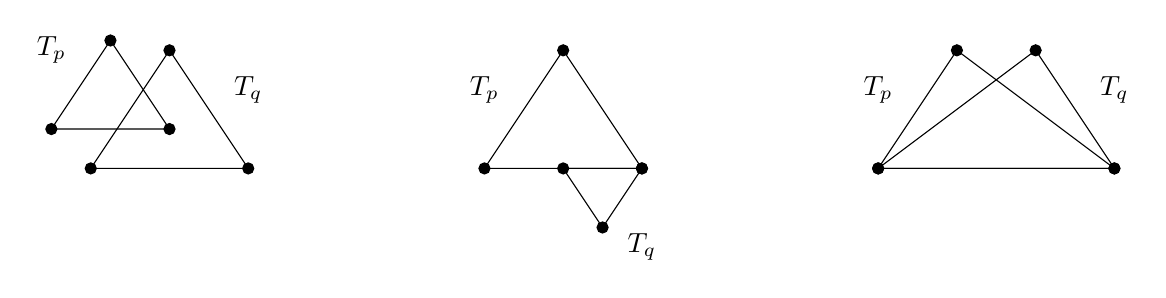
\begin{tikzpicture}
        % Figure 1
        \draw (0.5, 0.5) -- (1.25, 1.625) -- (2, 0.5) -- cycle;
        \filldraw[black] (0.5, 0.5) circle (2pt);
        \filldraw[black] (1.25, 1.625) circle (2pt);
        \filldraw[black] (2, 0.5) circle (2pt);
        \node at (0.5, 1.5) {$T_p$};
        
        \draw (1, 0) -- (2, 1.5) -- (3, 0) -- cycle;
        \filldraw[black] (1, 0) circle (2pt);
        \filldraw[black] (2, 1.5) circle (2pt);
        \filldraw[black] (3, 0) circle (2pt);
        \node at (3, 1){$T_q$};


        % Figure 2
        \draw (6, 0) -- (7, 1.5) -- (8, 0) -- cycle;
        \filldraw[black] (6, 0) circle (2pt);
        \filldraw[black] (7, 1.5) circle (2pt);
        \filldraw[black] (8, 0) circle (2pt);
        \node at (6, 1){$T_p$};

        \draw (7, 0) -- (8, 0) -- (7.5, -0.75) -- cycle;
        \filldraw[black] (7, 0) circle (2pt);
        \filldraw[black] (8, 0) circle (2pt);
        \filldraw[black] (7.5, -0.75) circle (2pt);
        \node at (8, -1){$T_q$};

        % Figure 3
        \draw (11, 0) -- (12, 1.5) -- (14, 0) -- cycle;
        \filldraw[black] (11, 0) circle (2pt);
        \filldraw[black] (12, 1.5) circle (2pt);
        \filldraw[black] (14, 0) circle (2pt);
        \node at (11, 1){$T_p$};

        \draw (11, 0) -- (13, 1.5) -- (14, 0) -- cycle;
        \filldraw[black] (11, 0) circle (2pt);
        \filldraw[black] (13, 1.5) circle (2pt);
        \filldraw[black] (14, 0) circle (2pt);
        \node at (14, 1){$T_q$};
    \end{tikzpicture}

    Admissible : \\
    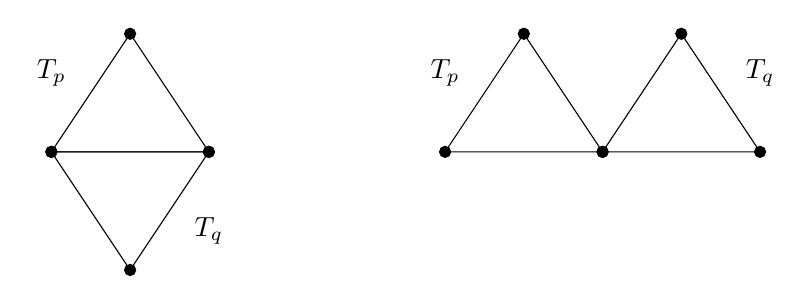
\begin{tikzpicture}
        % Figure 1
        \draw (0, 0) -- (1, 1.5) -- (2, 0) -- cycle;
        \filldraw[black] (0, 0) circle (2pt);
        \filldraw[black] (1, 1.5) circle (2pt);
        \filldraw[black] (2, 0) circle (2pt);
        \node at (0, 1){$T_p$};

        \draw (0, 0) -- (2, 0) -- (1, -1.5) -- cycle;
        \filldraw[black] (0, 0) circle (2pt);
        \filldraw[black] (2, 0) circle (2pt);
        \filldraw[black] (1, -1.5) circle (2pt);
        \node at (2, -1){$T_q$};

        % Figure 2
        \draw (5, 0) -- (6, 1.5) -- (7, 0) -- cycle;
        \filldraw[black] (5, 0) circle (2pt);
        \filldraw[black] (6, 1.5) circle (2pt);
        \filldraw[black] (7, 0) circle (2pt);
        \node at (5, 1){$T_p$};

        \draw (7, 0) -- (9, 0) -- (8, 1.5) -- cycle;
        \filldraw[black] (7, 0) circle (2pt);
        \filldraw[black] (9, 0) circle (2pt);
        \filldraw[black] (8, 1.5) circle (2pt);
        \node at (9, 1){$T_q$};
    \end{tikzpicture}

    \item . \\
    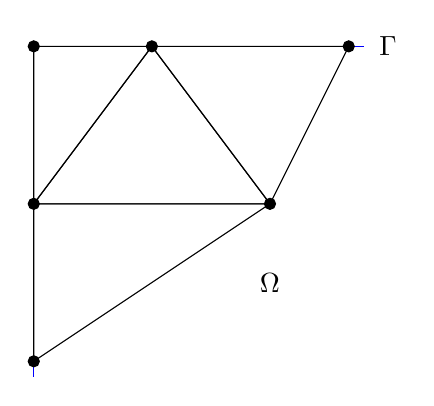
\begin{tikzpicture}
        \draw[blue] (0, 0) -- (4.2, 0);
        \draw[blue] (0, 0) -- (0, -4.2);
        \node at (4.5, 0) {$\Gamma$};

        \draw (0, 0) -- (1.5, 0) -- (0, -2) -- cycle;
        \draw (0, -2) -- (1.5, 0) -- (3, -2) -- cycle;
        \draw (1.5, 0) -- (4, 0) -- (3, -2) -- cycle;
        \draw (0, -2) -- (0, -4) -- (3, -2) -- cycle;

        \filldraw[black] (0, 0) circle (2pt);
        \filldraw[black] (1.5, 0) circle (2pt);
        \filldraw[black] (0, -2) circle (2pt);
        \filldraw[black] (3, -2) circle (2pt);
        \filldraw[black] (4, 0) circle (2pt);
        \filldraw[black] (0, -4) circle (2pt);

        \node at (3, -3) {$\Omega$};
    \end{tikzpicture}

    \item . \\
    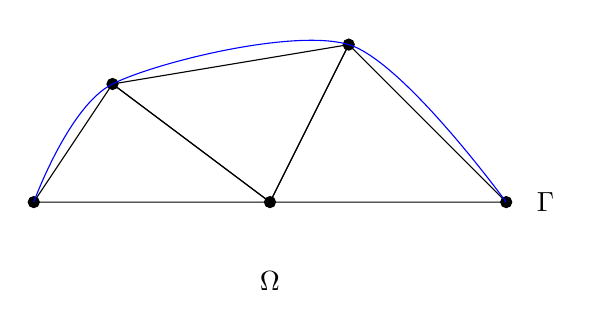
\begin{tikzpicture}
        \draw (0, 0) -- (1, 1.5) -- (3, 0) -- cycle;
        \draw (1, 1.5) -- (3, 0) -- (4, 2) -- cycle;
        \draw (3, 0) -- (4, 2) -- (6, 0) -- cycle;

        \filldraw[black] (0, 0) circle (2pt);
        \filldraw[black] (1, 1.5) circle (2pt);
        \filldraw[black] (3, 0) circle (2pt);
        \filldraw[black] (4, 2) circle (2pt);
        \filldraw[black] (6, 0) circle (2pt);

        \node at (3, -1) {$\Omega$};

        \draw[blue] plot [smooth] coordinates {(0, 0) (1, 1.5) (4, 2) (6, 0)};
        \node at (6.5, 0) {$\Gamma$};
    \end{tikzpicture}
\end{enumerate}


On suppose par la suite, par la convergence de la méthode, que \\
$\exists c > 0$ tel que $\forall h > 0, \underset{T \in \mathcal{T}_h}{\sup} \frac{\text{diam}(T)}{\mathcal{C}^{(T)}} \leq c$ avec $\mathcal{C}^{(T)}$ le rayon du cercle inscrit dans $T$. \\

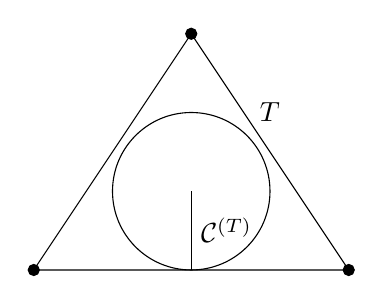
\begin{tikzpicture}
    \draw (0, 0) -- (2, 3) -- (4, 0) -- cycle;
    
    \draw (2, 1) circle (1cm);

    \filldraw[black] (0, 0) circle (2pt);
    \filldraw[black] (2, 3) circle (2pt);
    \filldraw[black] (4, 0) circle (2pt);

    \node at (3, 2) {$T$};

    \draw (2, 1) -- (2, 0) node[midway, right]{$\mathcal{C}^{(T)}$};

\end{tikzpicture}


\subsubsection{Exemple}

Soit $\Omega = ]0, 1[ \times ]0, 1[$. \\
On considère le problème suivant :
$\begin{cases}
    -\Delta u + u = f & \text{sur } \Omega \\
    u = 0 & \text{sur } \Gamma
\end{cases}$\\

On rappelle le problème $(P_{FV})$ : \\
Trouver $u \in H^1_0(\Omega)$ tel que $\forall v \in H^1_0(\Omega), a(u, v) = l(v)$ \\
avec $\begin{array}[t]{lrcl}
    a : & H^1_0(\Omega) \times H^1_0(\Omega) & \longrightarrow & \mathbb{R} \\
    & (u, v) & \longmapsto & \int_{\Omega} \nabla u \cdot \nabla v dx + \int_{\Omega} uv dx
\end{array}$ \\
et $\begin{array}[t]{lrcl}
    l : & H^1_0(\Omega) & \longrightarrow & \mathbb{R} \\
    & v & \longmapsto & \int_{\Omega} fv dx
\end{array}$\\
$(P_{FV})$ admet une solution unique (Théorème de Lax-Milgram). \\

On suppose avoir $N_T$ triangles et $\mathcal{T}_h = (T_p)_{p \in \llbracket 1, N_T \rrbracket}$ une triangulation admissible de $\Omega$. \\
On note $(q_i)_{i \in \llbracket 1, N_T \rrbracket}$ les sommets des triangles $T_p$. \\
On note $P^1 = \mathbb{R}_1[X_1, X_2]$ l'espace des polynômes de degré au plus 1 par rapport à $X_1$ et $X_2$.
On a donc $P^1 = \text{Vect}\{1, X_1, X_2\}$. \\

On pose $\tilde{V_h} = \{v \in \mathcal{C}^0(\overline{\Omega}), v_{|T_p} \in P^1, \forall p \in \llbracket 1, N_T \rrbracket\}$. \\
$V_h = \{v_h \in \tilde{V_h}, v_{h | \Gamma} = 0\}$. \\


\propriete{}{
    \begin{enumerate}[label=\roman*)]
        \item Les fonctions de $\tilde{V_h}$ sont entièremement définies par leurs valeurs en leurs sommets $q_i$.
        \item $\dim \tilde{V_h} = N_S$. \\
        De plus, une base de $\tilde{V_h}$ est donnée par $(\varphi_i)_{i \in \llbracket 1, N_S \rrbracket}$ avec $\varphi_i(q_j) = \delta_{ij}$. \\
        En particulier, $\forall v_h \in \tilde{V_h}, v_h = \sum_{i=1}^{N_S} v_h(q_i) \varphi_i$.
        \item $\tilde{V_h} \subset H^1(\Omega)$.
        \item $\dim V_h = N_1$ avec $N_1$ le nombre de sommets $q_i$ n'appartenant pas à $\Gamma$.
        \item $V_h \subset H^1_0(\Omega)$.
    \end{enumerate}
}

\remarque{
    shema
}


\preuve{
    \textit{Texte Manquant}
}


Pour résoudre le problème $(P_{FV})$, il nous faut résoudre le système linéaire $Ax = b$ avec $\forall (i, j) \in \llbracket 1, N_S \rrbracket^2, A_{ij} = a(\varphi_i, \varphi_j)$ et $b_i = l(\varphi_i)$. $u_h = \sum_{i=1}^{N_S} x_i \varphi_i$. \\


\underline{Construction de $A$ et $b$ :} \\
On a : $a(\varphi_i, \varphi_j) = \int_{\Omega} \nabla \varphi_i \cdot \nabla \varphi_j dx + \int_{\Omega} \varphi_i \varphi_j dx$. \\
et $b_i = l(\varphi_i) = \int_{\Omega} f \varphi_i dx$. \\

$A_{ij} = \sum_{p=1}^{N_T} \left[ \int_{T_p} \nabla \varphi_i \cdot \nabla \varphi_j dx + \int_{T_p} \varphi_i \varphi_j dx \right]$ : on se ramène sur des intégrales sur les triangles du maillage $\mathcal{T}_h$. \\

\begin{itemize}
    \item \underline{$1^{er}$ cas :} $\lambda (\text{supp}(\varphi_i) \cap \text{supp}(\varphi_j)) = 0$ \\
    $\Rightarrow \int_{\Omega} \varphi_i \varphi_j dx = 0$ et $\int_{\Omega} \nabla \varphi_i \cdot \nabla \varphi_j dx = 0 \Rightarrow A_{ij} = 0$.
    \item \underline{$2^{eme}$ cas :} $\lambda (\text{supp}(\varphi_i) \cap \text{supp}(\varphi_j)) \neq 0$ \\
    Calcul de $\int_{\Omega} \nabla \varphi_i \cdot \nabla \varphi_j dx + \int_{\Omega} \varphi_i \varphi_j dx$ : stratégie de l'élément de référence. \\

    $T_p = \left[ q_i, q_j, q_l \right]$, $\{ii, jj, ll\} = \{1, 2, 3\}^2$. \\
    Sur $T_p$, on s'intéresse à $\varphi_i, \varphi_j, \varphi_l$ uniquement. \\
    $\Rightarrow$ Changeons de variables pour se ramener à un domaine d'intégration "simple". \\

    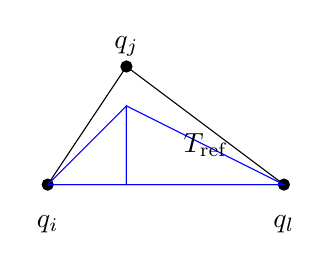
\begin{tikzpicture}
        \draw (0, 0) -- (1, 1.5) -- (3, 0) -- cycle;
        \filldraw[black] (0, 0) circle (2pt);
        \filldraw[black] (1, 1.5) circle (2pt);
        \filldraw[black] (3, 0) circle (2pt);

        \node at (0, -0.5) {$q_i$};
        \node at (1, 1.75) {$q_j$};
        \node at (3, -0.5) {$q_l$};

        \draw[blue] (0, 0) -- (1, 0) -- (1, 1) -- (0, 0);
        \draw[blue] (1, 0) -- (3, 0) -- (1, 1) -- (1, 0);

        \node at (2, 0.5) {$T_{\text{ref}}$};
    \end{tikzpicture}

    avec $\Phi$ affine de sorte que $\Phi_{T_p}(A^{(k)}) = A_p^{(kk)} \quad k \in \llbracket 1, 3 \rrbracket, kk \in \llbracket ii, jj, ll \rrbracket$. \\ 
\end{itemize}


\definition{- Coordonnées barycentriques relatives à un triangle}{
    Soit $T = [A^{(1)}, A^{(2)}, A^{(3)}]$ un triangle. \\
    $\forall M = (x_1, x_2) \in \mathbb{R}^2$, $\exists! (\lambda_i(M))_{i \in \llbracket 1, 3 \rrbracket} \in \mathbb{R}^3 \text{ tel que }$ : \\
    $M = \sum_{i=1}^3 \lambda_i(M) A^{(i)} \text{ et } \sum_{i=1}^3 \lambda_i(M) = 1$. \\

    Les $\lambda_i(M)$ sont appellées les \textit{coordonnées barycentriques} de $M$ relatives à $T$. \\

    De plus, on a :
    \begin{enumerate}[label=\roman*)]
        \item $\forall (i, j) \in \llbracket 1, 3 \rrbracket^2, \lambda_i(A^{(j)}) = \delta_{ij}$.
        \item $\forall M \in (A^{(i)}, A^{(j)})$ avec $(i, j) \in \llbracket 1, 3 \rrbracket^2, i \neq j \Rightarrow \lambda_k(M) > 0$.
        \item $\forall M \in T, \forall i \in \llbracket 1, 3 \rrbracket, 0 \leq \lambda_i(M) \leq 1$.
    \end{enumerate}
}


\underline{Expression de $\Phi_{T_p}(M)$ :}
\begin{align*}
    \Phi_{T_p}(M) &= A_p^{(ii)} + x_1 \overrightarrow{A_p^{(ii)} A_p^{(jj)}} + x_2 \overrightarrow{A_p^{(ii)} A_p^{(ll)}} \hspace{14.5cm} \\
    &= A_p^{(ii)} + x_1 (A_p^{(jj)} - A_p^{(ii)}) + x_2 (A_p^{(ll)} - A_p^{(ii)}) \\
    &= (1 - x_1 - x_2) A_p^{(ii)} + x_1 A_p^{(jj)} + x_2 A_p^{(ll)}
\end{align*}

On pose $\lambda_i(M) = 1 - x_1 - x_2, \lambda_j(M) = x_1, \lambda_l(M) = x_2$. \\
On a $\sum_{i=1}^3 \lambda_i(M) = 1$. \\
Donc $(\lambda_i)_{i \in \llbracket 1, 3 \rrbracket}$ sont les coordonnées barycentriques de $\Phi_{T_p}(M)$ relatives à $T_p$. \\

Pour le triangle de référence $T_u$ : \\
$\forall M \in T_u, \forall k \in \{ii, jj, ll\}, \lambda_k^{(T_p)}(\Phi_{T_p}(M)) = \lambda_k^{(T_u)}(M)$. \\

Sur $T_p$, $\lambda_{ii}^{(T_p)}(A_p^{(kk)}) = \delta_{ii, kk} = \varphi_i(A_p^{(kk)}) = \varphi_i(q_k)$. \\
et $\lambda_{ii}^{(T_p)}(M) = \varphi_i(M)$. \\

Avec $q_i, q_j$ des sommets de $T_p$, on a : \\
$\int_{T_p} \varphi_i \varphi_j dx = \int_{T_p} \lambda_{ii}^{(T_p)} \lambda_{jj}^{(T_p)} dx = \int_{T_u} (\lambda_{ii}^{(T_p)} \circ \Phi_{T_p})(\lambda_{jj}^{(T_p)} \circ \Phi_{T_p}) |J_{\Phi_{T_p}}| dx = \int_{T_u} \lambda_{ii}^{(T_u)} \lambda_{jj}^{(T_u)} |J_{\Phi_{T_p}}| dx$. \\
avec $|J_{\Phi_{T_p}}| = \| \overrightarrow{A_p^{(ii)} A_p^{(jj)}} \cap \overrightarrow{A_p^{(ii)} A_p^{(ll)}} \| = 2 \times aire(T_p)$. \\

$\int_{T_p} \varphi_i \varphi_j dx = 2 \times aire(T_p) \int_{0}^{1} \int_{0}^{1 - x_2} \lambda_{ii}^{(T_u)} \lambda_{jj}^{(T_u)} dx_1 dx_2 = 2 \times aire(T_p) \int_{0}^{1} x_2 \left( \int_{0}^{1 - x_2} x_1 dx_1 \right) dx_2$. \\
$\Rightarrow \int_{T_p} \varphi_i \varphi_j dx = \frac{aire(T_p)}{12}$. \\



\begin{algorithm}[H]
    \caption{Assemblage de la matrice $A$ et du vecteur $b$}
    \textbf{For :} $p = 1, N_T$ \# Boucle sur les triangles $T_p= [q_i, q_j, q_l] = [A_p^{(ii)}, A_p^{(jj)}, A_p^{(ll)}]$ \\
    \vspace{0.5cm}
    \hspace{0.5cm} $\bullet$ \textbf{Calcul de $M_{T_p} \in \mathcal{M}_2(\mathbb{R})$} \\
    \hspace{0.5cm} $\left[ M_{T_p} \right]_{ii, ii} = \int_{T_p} \nabla \varphi_i \cdot \nabla \varphi_i dx + \int_{T_p} \varphi_i \varphi_i dx$ \\
    \vspace{0.5cm}
    \hspace{0.5cm} $\bullet$ \textbf{Mise à jour de $A$} \\
    \hspace{0.5cm} $A(\left[q_i, q_j, q_l\right], \left[q_i, q_j, q_l\right]) = A(\left[q_i, q_j, q_l\right], \left[q_i, q_j, q_l\right]) + M_{T_p}$ \\
    \vspace{0.5cm}
    \hspace{0.5cm} $\bullet$ \textbf{Calcul de $T_0 \in \mathbb{R}^3$} \\
    \hspace{0.5cm} $T_{0, ii} = \int_{T_p} f q_i dx$ \\
    \vspace{0.5cm}
    \hspace{0.5cm} $\bullet$ \textbf{Mise à jour de $b$} \\
    \hspace{0.5cm} $b(\left[q_i, q_j, q_l\right]) = b(\left[q_i, q_j, q_l\right]) + T_0$ \\
    \vspace{0.5cm}
    \textbf{End For}  
\end{algorithm}




\end{document}
